\subsection{Theory and Procedure}

\FloatBarrier

\begin{figure}[h!]
	\centering
	\caption{Common-Source Amplifier}
	\label{fig:cs_amp}
	\begin{circuitikz}
		\draw
		( 0 , 0 ) node[ nmos ] (my_nmos) {}

		% Gate
		(my_nmos.G) to [ short ] ++( -2 , 0 ) coordinate(g_out)
		(g_out) to [V , v=$V_{in}$ ] ++( 0 , -2 ) coordinate(gnd_1)
		(gnd_1) node[ ground ] (my_gnd_1) {}

		% Drain
		(my_nmos.D) node[label={[font=\footnotesize]0:$V_{out}$}] {} 
		to [ R={$5k\Omega$} ] ++( 0, 2 ) coordinate(labeled_D)
		(labeled_D) to [ short ] ++( 2, 0) coordinate(vcc)
		(vcc) to [ V , v=$V_{DD}\rightarrow5V$ ] ++( 0 , -3 ) coordinate(gnd_3)
		(gnd_3) node[ ground ] (my_gnd_3) {}

		% Source
		(my_nmos.S) node [ ] (S) {}
		(S) to [ short ] ++( 0 , -1 ) coordinate(my_e_gnd)
		(my_e_gnd) node[ ground ] (e_gnd) {}

		;
	\end{circuitikz}
\end{figure}

\FloatBarrier

The common-source amplifier pictured above is then constructed.
$V_{in}$ is again swept from $0$\si{\volt} to $5$\si{\volt}.
In the common-source arrangement, the NMOS transistor has the following condition for saturation:

\begin{equation}
	\label{eq:sat_cond_nmos_csa}
	V_{DS} > V_{GS} - V_T \rightarrow V_{out} = 5V - I_{D}R > V_{in} - V_T \rightarrow V_{in} < 5V - I_{D}R + V_T
\end{equation}

In the common-source arrangement, $V_{in}$ is equivalent to $V_{GS}$.
So, when $V_{in}$ is less than the threshold voltage, the transistor operates in the cutoff region and no current is passed through the transistor and consequently, the resistor.
Because the transistor effectively acts as an open circuit, $V_{out}$ is equivalent to $V_{DD}$ for the entirety of the cutoff region.
When $V_{in}$ begins to overtake the threshold voltage, the transistor immediately operates in the saturation region.
This is because small values of $V_{GS}$ yield small $I_{D}$ and thus, the condition in equation (\ref{eq:sat_cond_nmos_csa}) is met.
As $V_{in}$ gets larger, $I_{D}$ will also increase and $V_{out}$ will decrease as a result.
When $V_{in}$ becomes sufficiently large, $I_{D}$ will be large enough to violate the saturation condition and the transistor will then operate in triode mode.
In triode region, $V_{out}$ is expected to be very small because of the large $I_{D}$. \\

\subsection{Results}

\FloatBarrier

\begin{figure}[h!]
	\centering
	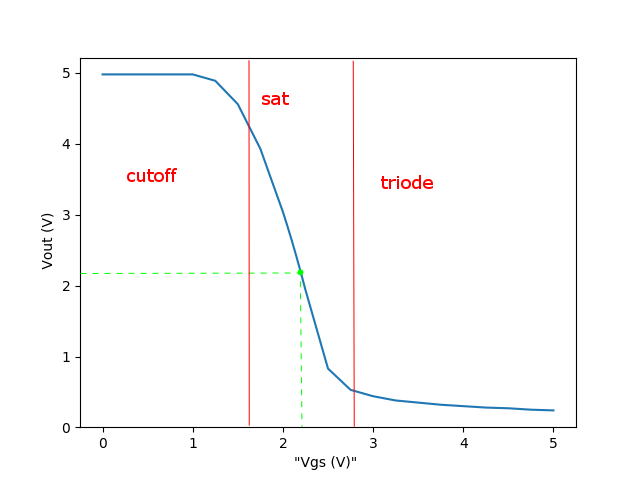
\includegraphics[scale=0.75]{./data/common_source_edited.png}
	\caption{Common Source Amplifier Voltage Transfer Characteristic}
	\label{fig:common_source}
\end{figure}

\FloatBarrier

The threshold voltage $V_T$ is again taken to be $1.7$\si{\volt}.
So, the NMOS transistor operates in the cutoff region when $V_{in} < 1.7$\si{\volt} and $V_{out} = 5$\si{\volt} for the majority of this range.
When $V_{in} > 1.7$\si{\volt}, the transistor enters saturation mode and $V_{O}$ sharply decreases. \\
Then, the bias point occurs when the following condition is met:

\begin{equation}
	\label{eq:bias_nmos_csa}
	V_{DS} = V_{DD} - I_{D}R \rightarrow V_{in} = 5V - I_{D}R = V_{out}
\end{equation}

Following the condition above, the bias point occurs at $V_{in} = V_{out} \approx 2.2V$ according to results shown in Figure (\ref{fig:common_source}).
This voltage corresponds to the bias current $I_{D} = \frac{V_{out}}{5k\Omega} \approx \frac{2.2V}{5k\Omega} = 0.44$\si{\milli\ampere}.
The transistor enters triode mode when $V_{in}$ exceeds $5V - I_{D}R + V_T$, which is beyond the bias point.
With the assumption that the bias point occurs at the midpoint between the saturation and triode boundaries, $V_{in}$ at triode region can be approximated to be $2.2V + (2.2V - 1.7V) \approx 2.7V$.

